\documentclass[10pt]{beamer}
\usetheme[
%%% options passed to the outer theme
%    hidetitle,           % hide the (short) title in the sidebar
%    hideauthor,          % hide the (short) author in the sidebar
%    hideinstitute,       % hide the (short) institute in the bottom of the sidebar
%    shownavsym,          % show the navigation symbols
%    width=2cm,           % width of the sidebar (default is 2 cm)
%    hideothersubsections,% hide all subsections but the subsections in the current section
%    hideallsubsections,  % hide all subsections
%    left                % right of left position of sidebar (default is right)
  ]{Aalborg}
  
% If you want to change the colors of the various elements in the theme, edit and uncomment the following lines
% Change the bar and sidebar colors:
%\setbeamercolor{Aalborg}{fg=red!20,bg=red}
%\setbeamercolor{sidebar}{bg=red!20}
% Change the color of the structural elements:
%\setbeamercolor{structure}{fg=red}
% Change the frame title text color:
%\setbeamercolor{frametitle}{fg=blue}
% Change the normal text color background:
%\setbeamercolor{normal text}{bg=gray!10}
% ... and you can of course change a lot more - see the beamer user manual.

\usepackage[utf8]{inputenc}
\usepackage[spanish]{babel}
\usepackage[T1]{fontenc}
% Or whatever. Note that the encoding and the font should match. If T1
% does not look nice, try deleting the line with the fontenc.

\usepackage[table,xcdraw]{xcolor}
\usepackage{helvet}
\usepackage{tikz}
\usetikzlibrary{shapes,arrows,positioning}

\usepackage{minted}


\usepackage{listings}
\usepackage{color}
\definecolor{codegreen}{rgb}{0,0.6,0}
\definecolor{codegray}{rgb}{0.5,0.5,0.5}
\definecolor{codepurple}{rgb}{0.58,0,0.82}
\definecolor{backcolour}{rgb}{0.95,0.95,0.92}
 
\lstdefinestyle{mystyle}{
    backgroundcolor=\color{backcolour},   
    commentstyle=\color{codegreen},
    keywordstyle=\color{magenta},
    numberstyle=\tiny\color{codegray},
    stringstyle=\color{codepurple},
    basicstyle=\footnotesize,
    breakatwhitespace=false,         
    breaklines=true,                 
    captionpos=b,                    
    keepspaces=true,                 
    numbers=left,                    
    numbersep=5pt,                  
    showspaces=false,                
    showstringspaces=false,
    showtabs=false,                  
    tabsize=2
}
 
\lstset{style=mystyle}


% colored hyperlinks
\newcommand{\chref}[2]{%
  \href{#1}{{\usebeamercolor[bg]{Aalborg}#2}}%
}

\title[Servomecanismos]% optional, use only with long paper titles
{Servomecanismos}

%\title[Sensores y Actuadores]% optional, use only with long paper titles
%{Sensores y Actuadores}

%\title[Percepción]% optional, use only with long paper titles
%{Percepción}

\subtitle{Git y Github para poetas, parte 5}  % could also be a conference name

\date{\today}

\author[Víctor Medrano Zarazúa] % optional, use only with lots of authors
{
  Víctor Medrano Zarazúa\\
  \href{mailto:victor.medranozr@uanl.edu.mx}{{\tt victor.medranozr@uanl.edu.mx}}
}
% - Give the names in the same order as they appear in the paper.
% - Use the \inst{?} command only if the authors have different
%   affiliation. See the beamer manual for an example

\institute[
%  {\includegraphics[scale=0.2]{aau_segl}}\\ %insert a company, department or university logo
  %Dept.\ of Electronic Systems\\
  Universidad Autónoma de Nuevo León\\
  Facultad de Ingeniería Mecánica y Eléctrica
] % optional - is placed in the bottom of the sidebar on every slide
{% is placed on the bottom of the title page
  %Department of Electronic Systems\\
  Universidad Autónoma de Nuevo León\\
  Facultad de Ingeniería Mecánica y Eléctrica
  
  %there must be an empty line above this line - otherwise some unwanted space is added between the university and the country (I do not know why;( )
}

% specify the logo in the top right/left of the slide
\pgfdeclareimage[height=1cm]{mainlogo}{AAUgraphics/FIME} % placed in the upper left/right corner
\logo{\pgfuseimage{mainlogo}}

% specify a logo on the titlepage (you can specify additional logos an include them in 
% institute command below
\pgfdeclareimage[height=1.5cm]{titlepagelogo}{AAUgraphics/UANL} % placed on the title page
%\pgfdeclareimage[height=1.5cm]{titlepagelogo2}{AAUgraphics/aau_logo_new} % placed on the title page
\titlegraphic{% is placed on the bottom of the title page
  \pgfuseimage{titlepagelogo}
%  \hspace{1cm}\pgfuseimage{titlepagelogo2}
}

%\definecolor{UniBlue}{RGB}{255,255,255}

\tikzset{
block/.style={
  draw, 
  fill=blue!20, 
  rectangle, 
  minimum height=3em, 
  minimum width=6em
  },
 gain/.style={
    draw,
    fill=blue!20, 
    isosceles triangle,
    minimum height = 3em,
    isosceles triangle apex angle=60
    },
sum/.style={
  draw, 
  fill=blue!20, 
  circle, 
  },
input/.style={coordinate},
output/.style={coordinate},
pinstyle/.style={
  pin edge={to-,thin,black}
  }
}  

\begin{document}
% the titlepage


%\setbeamercolor{title}{fg=UniBlue}
%\setbeamercolor{normal text}{fg=UniBlue}
%\setbeamercolor{Aalborg}{fg=black,bg=black}


{\aauwavesbg
\begin{frame}[plain,noframenumbering] % the plain option removes the sidebar and header from the title page
  \titlepage
\end{frame}}
%%%%%%%%%%%%%%%%

% TOC
\begin{frame}{Contenido}{}
\tableofcontents
\end{frame}
%%%%%%%%%%%%%%%%
\section{Repaso}
\begin{frame}{Repaso}{}
\begin{block}{Recapítulemos...}
\begin{itemize}
    \item ¿Qué es la terminal/bash?
    \item ¿Cuál es la diferencia entre Git y Github?
    \item ¿Cuáles son los comandos principales Unix/Linux a ejecutar en la terminal?
    \item ¿Qué comandos hemos visto para administrar repositorios por medio de Git?
    \item ¿Cuál es la diferencia entre repositorio local/remoto?
    \item ¿Cuál es la diferencia entre push/pull?
\end{itemize}
\end{block}

%\begin{figure}[h!]
%\centering
%
\includegraphics [scale=0.32]{github}
%\caption{Bobina Tesla}
%\label{fig:tesla}
%\end{figure}

\end{frame}

\section{Introducción}

\begin{frame}{Introducción}{}
\begin{block}{Más sobre la terminal y Git}
\medskip
\begin{columns}[c]
\column{2in}
\begin{itemize}
    \item Veremos más comandos básicos para la terminal. 
    \item Veremos más comandos básicos de git para crear repositorios y agregar archivos.
\end{itemize}

\column{1.5in}
\framebox{
\includegraphics[width=1.5in]{terminal.png}}
\end{columns}
\end{block}
\end{frame}

\section{Más sobre la terminal}

\begin{frame}{Terminal}{Más comandos chidoris}

\begin{block}{}

%\begin{columns}[c]
\begin{itemize}
        \item mkdir (crea un nuevo directorio)
        \item rmdir (borra un directorio, solo si está vacío)
        \item rm (borra archivos o directorios)
        \item cp (copia archivos o directorios)
        \item touch (crea archivos)
        \item nano (abre editor de archivos en la terminal)
        \item cat (muestra el contenido de un archivo)
\end{itemize}
    
\end{block}

\end{frame}

\begin{frame}{Terminal}{GNU Nano}

\begin{block}{Editor de texto/código}

%\begin{columns}[c]
Podemos usar un editor de texto en la terminal para modificar archivos haciendo uso del comando \textcolor{blue}{nano}. Usaremos Ctrl + O para guardar los cambios y Ctrl + X para salir de editor.



\begin{figure}[h!]
\centering
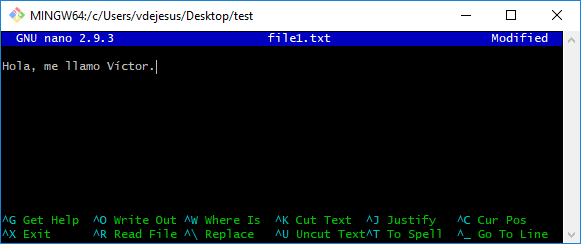
\includegraphics [scale=0.55]{nano}
%\caption{Sección de Issues}
\label{fig:git}
\end{figure}

\end{block}

\end{frame}

\section{Más sobre git}

\begin{frame}{Git}{Creación de un repositorio}

\begin{block}{Supongamos que...}

%\begin{columns}[c]
Has estado trabajando en un proyecto por una hora, una semana, un mes o un año y repentinamente necesitas convertir este proyecto en un repositorio local de Git y posteriormente alojarlo en un repositorio remoto de Github.

\begin{figure}[h!]
\centering

\includegraphics [scale=0.26]{elproyecto}
%\caption{Sección de Issues}
\label{fig:gitclone}
\end{figure}

\end{block}

\end{frame}

\begin{frame}{Git}{Más comandos de Git}

\begin{block}{}

%\begin{columns}[c]
\begin{itemize}
        \item git init
        \item git add
\end{itemize}
    
\end{block}

\end{frame}

\begin{frame}{Git}{Trabajando de forma local}

\begin{block}{Creando directorio e inicializando un repositorio local}

%\begin{columns}[c]
%Hacemos uso del comando git clone.

\begin{figure}[h!]
\centering
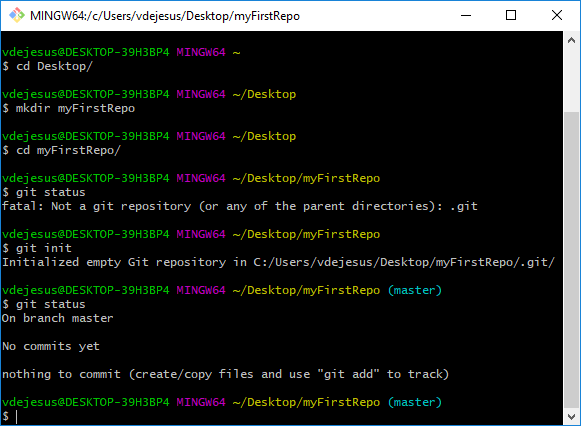
\includegraphics [scale=0.5]{step1}
%\caption{Sección de Issues}
\label{fig:gitclone2}
\end{figure}

\end{block}

\end{frame}

\begin{frame}{Git}{Trabajando de forma local}

\begin{block}{Creando archivos de texto}
Agregamos dos archivos de texto vacíos. Al verificar el status del repositorio nos menciona que hay dos archivos sin rastrear.
%\begin{columns}[c]
%Hacemos uso del comando git clone.

\begin{figure}[h!]
\centering
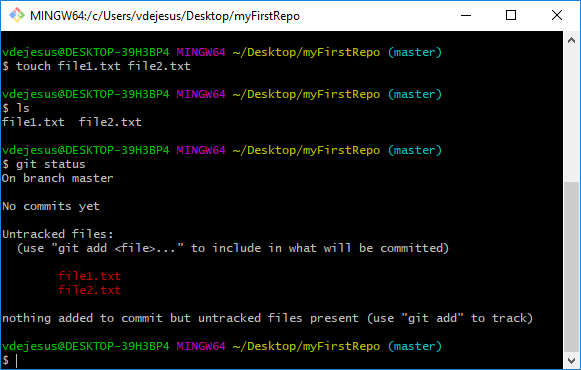
\includegraphics [scale=0.5]{step2}
%\caption{Sección de Issues}
\label{fig:gitclone3}
\end{figure}

\end{block}

\end{frame}

\begin{frame}{Git}{Trabajando de forma local}

\begin{block}{Agregando archivos al repositorio}
%\begin{columns}[c]
%Hacemos uso del comando git clone.

\begin{figure}[h!]
\centering
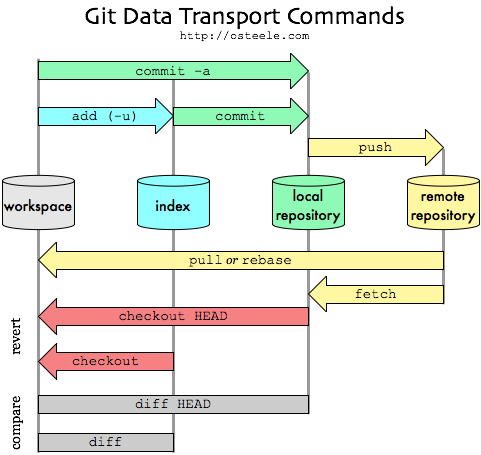
\includegraphics [scale=0.4]{addcommitpush}
%\caption{Sección de Issues}
\label{fig:gitstatus}
\end{figure}

\end{block}

\end{frame}

\begin{frame}{Git}{Trabajando de forma local}

\begin{block}{Agregando archivos al repositorio}

Cuando se crea un archivo por primera vez y queremos que sus modificaciones sean tomadas en cuenta por el repositorio local de git, usaremos el comando \textcolor{blue}{git add}. Este comando agrega archivos al index. 
%\begin{columns}[c]
%Hacemos uso del comando git clone.

\begin{figure}[h!]
\centering
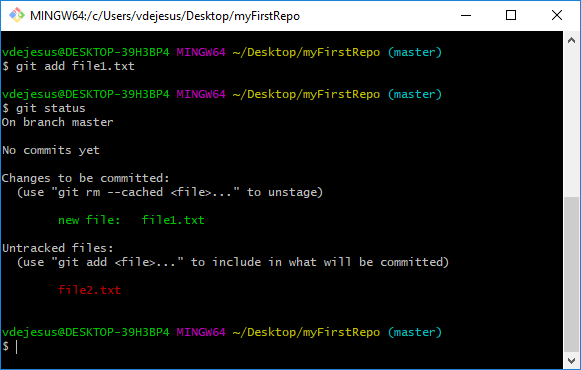
\includegraphics [scale=0.5]{step3}
%\caption{Sección de Issues}
\label{fig:gitstatus}
\end{figure}

\end{block}

\end{frame}

\begin{frame}{Git}{Trabajando de forma local}

\begin{block}{Agregando archivos al repositorio}
%\begin{columns}[c]
%Hacemos uso del comando git clone.
\begin{figure}[h!]
\centering
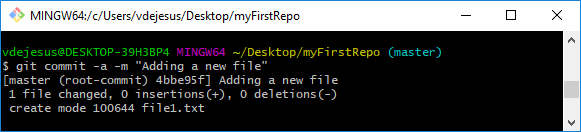
\includegraphics [scale=0.5]{step4_1}
%\caption{Sección de Issues}
\label{fig:gitstatus}
\end{figure}

\begin{figure}[h!]
\centering
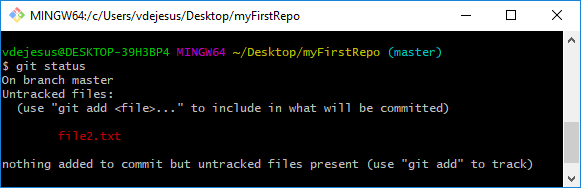
\includegraphics [scale=0.5]{step4_2}
%\caption{Sección de Issues}
\label{fig:gitstatus}
\end{figure}

\end{block}

\end{frame}


\begin{frame}{Git}{Haciendo push}

\begin{block}{Todo parecía perfecto hasta que...}
%\begin{columns}[c]
%Hacemos uso del comando git clone.
\begin{figure}[h!]
\centering
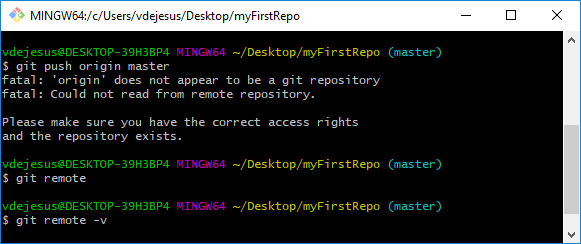
\includegraphics [scale=0.5]{sad}
%\caption{Sección de Issues}
\label{fig:gitstatus}
\end{figure}

\end{block}

\end{frame}

\begin{frame}{Git}{Haciendo push}

\begin{block}{Resolviendo el problema}
Creamos un nuevo repositorio en Github como lo hemos hecho anteriormente. Esta vez sin incluir un archivo \textit{README.md}.
\begin{figure}[h!]
\centering
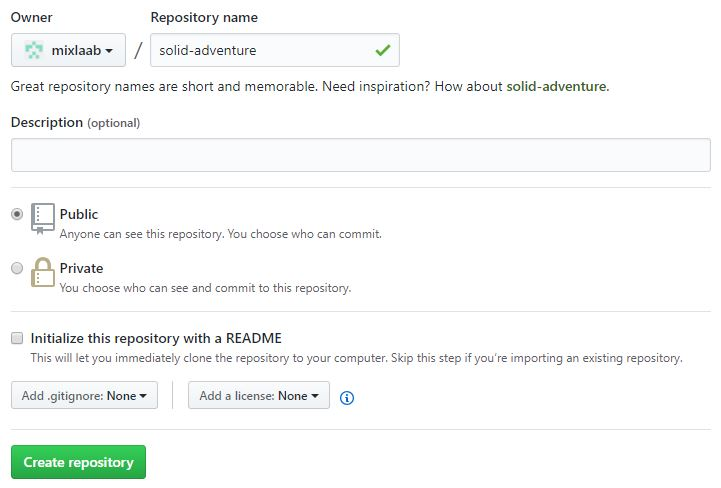
\includegraphics [scale=0.45]{step5}
%\caption{Sección de Issues}
\label{fig:gitstatus}
\end{figure}

\end{block}

\end{frame}

\begin{frame}{Git}{Haciendo push}

\begin{block}{Resolviendo el problema}
Copiamos el enlace que aparece en la página después de crear el repositorio.
\begin{figure}[h!]
\centering
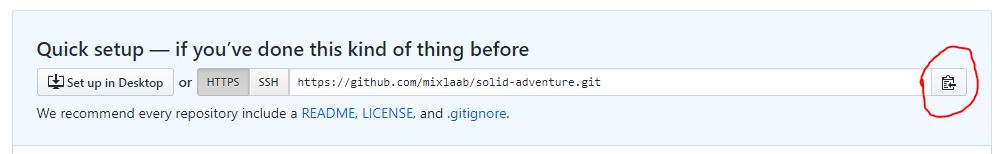
\includegraphics [scale=0.36]{step6}
%\caption{Sección de Issues}
\label{fig:gitstatus}
\end{figure}

\end{block}

\end{frame}

\begin{frame}{Git}{Haciendo push}

\begin{block}{Resolviendo el problema}
Pegamos el enlace para agregar un remoto y hacemos push al repositorio remoto.

\begin{figure}[h!]
\centering
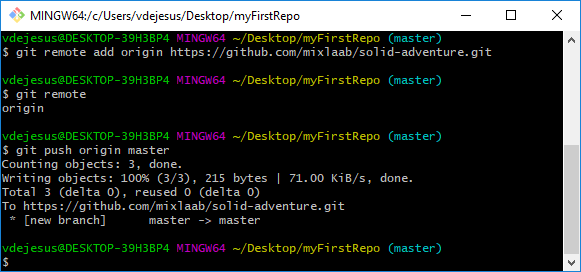
\includegraphics [scale=0.5]{step7}
%\caption{Sección de Issues}
\label{fig:gitstatus}
\end{figure}

\end{block}

\end{frame}

\begin{frame}{Git}{Haciendo push}

\begin{block}{Verificando que el push se ha hecho}

\begin{figure}[h!]
\centering
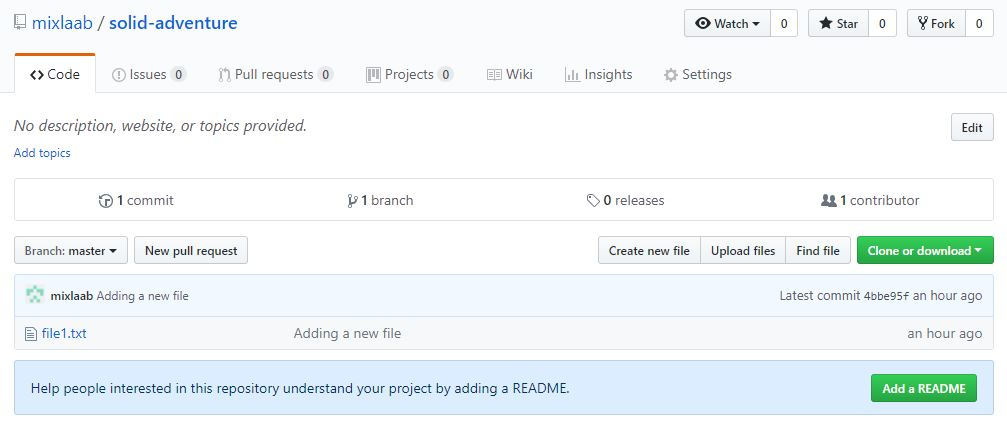
\includegraphics [scale=0.35]{step8}
%\caption{Sección de Issues}
\label{fig:gitstatus}
\end{figure}

\end{block}

\end{frame}

\begin{frame}{Git}{Haciendo pull}

\begin{block}{Modificando archivo en Github}
Modificamos \textit{file1.txt} en el repositorio remoto y hacemos commit.

\begin{figure}[h!]
\centering
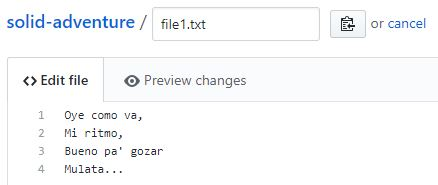
\includegraphics [scale=0.35]{step9}
%\caption{Sección de Issues}
\label{fig:gitstatus}
\end{figure}

\begin{figure}[h!]
\centering
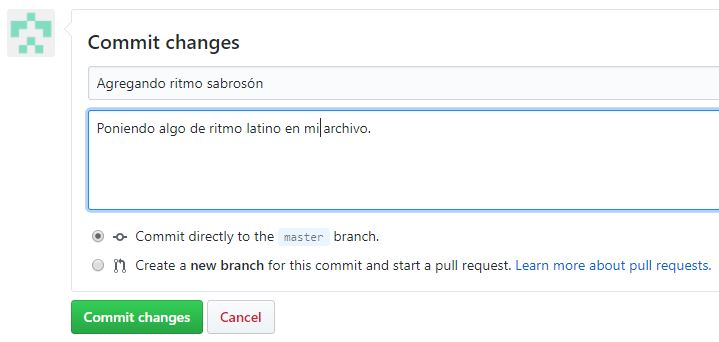
\includegraphics [scale=0.35]{step10}
%\caption{Sección de Issues}
\label{fig:gitstatus}
\end{figure}

\end{block}

\end{frame}

\begin{frame}{Git}{Haciendo pull}

\begin{block}{Actualizando repositorio local}
Hacemos pull al repositorio local con el comando \textcolor{blue}{git pull}

\begin{figure}[h!]
\centering
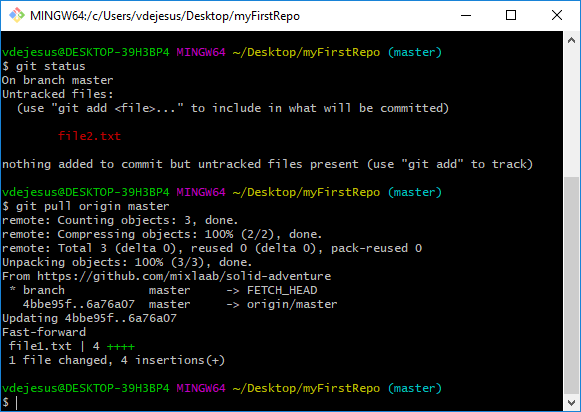
\includegraphics [scale=0.5]{step11}
%\caption{Sección de Issues}
\label{fig:gitstatus}
\end{figure}

\end{block}

\end{frame}

\begin{frame}{Git}{Haciendo pull}

\begin{block}{Verificando que el pull se ha hecho}

\begin{figure}[h!]
\centering
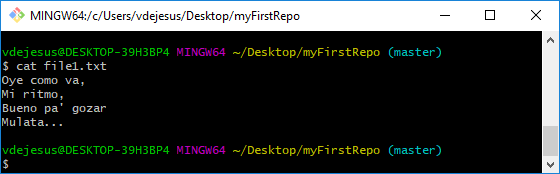
\includegraphics [scale=0.5]{step12}
%\caption{Sección de Issues}
\label{fig:gitstatus}
\end{figure}

\end{block}

\end{frame}

\section{En resumen}

\begin{frame}{En resumen}{}

%\begin{block}{Verificando que el pull se ha hecho}

\begin{figure}[h!]
\centering
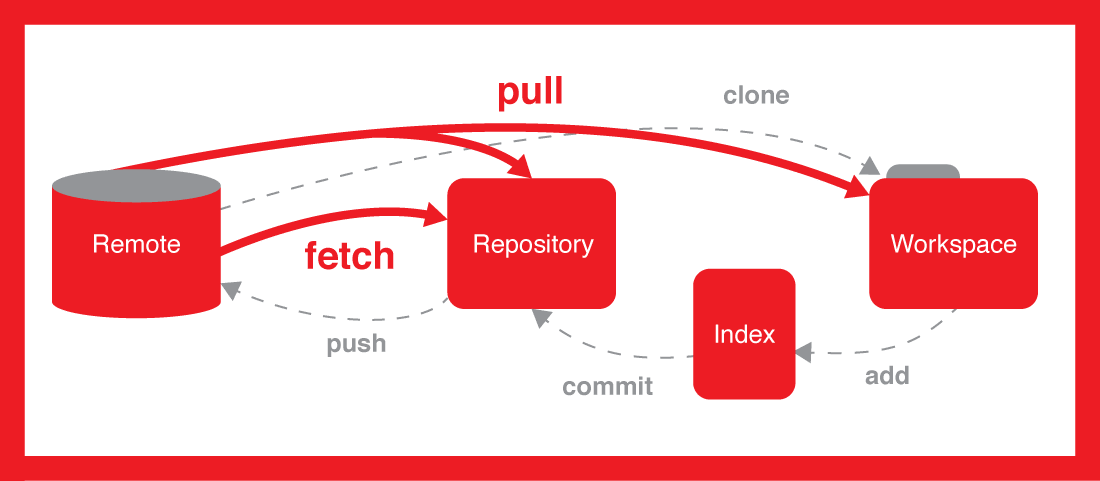
\includegraphics [scale=0.25]{gitnutshell}
%\caption{Sección de Issues}
\label{fig:gitstatus}
\end{figure}

%\end{block}

\end{frame}

\section{Información de contacto}
% contact information
\begin{frame}{Feedback}{Información de contacto}
En caso de comentarios, sugerencias, preguntas o errores en las diapositivas no dudes en contactarme.
  \begin{center}
    \insertauthor\\
    \chref{https://mixlaab.github.io}{https://mixlaab.github.io}\\
    WA: 8119022700\\
    %9220 Aalborg Ø
  \end{center}
\end{frame}
%%%%%%%%%%%%%%%%

{\aauwavesbg%
\begin{frame}[plain,noframenumbering]%
  \finalpage{Fin}
\end{frame}}
%%%%%%%%%%%%%%%%

\end{document}
